\documentclass[14pt, fleqn, xcolor={dvipsnames, table}]{beamer}
\usepackage[T2A]{fontenc}
\usepackage[utf8]{inputenc}
\usepackage[english,russian]{babel}
\usepackage{amssymb,amsfonts,amsmath,mathtext}
\usepackage{cite,enumerate,float,indentfirst}
\usepackage{cancel}
\usepackage{graphicx}
\usepackage{animate}

\usepackage{tikz}
% \usepackage{enumitem}
\usetikzlibrary{shadows}

% \usepackage{enumitem}
% \setitemize{label=\usebeamerfont*{itemize item}%
%   \usebeamercolor[fg]{itemize item}
%   \usebeamertemplate{itemize item}}

\graphicspath{{images/}}

\usetheme{Madrid}
\usecolortheme{seahorse}
\renewcommand{\CancelColor}{\color{red}}

\setbeamercolor{footline}{fg=Blue!50}
\setbeamertemplate{footline}{
  \leavevmode%
  \hbox{%
  \begin{beamercolorbox}[wd=.333333\paperwidth,ht=2.25ex,dp=1ex,center]{}%
    И. Кураленок, Н. Поваров, Яндекс
  \end{beamercolorbox}%
  \begin{beamercolorbox}[wd=.333333\paperwidth,ht=2.25ex,dp=1ex,center]{}%
    Санкт-Петербург, 2013
  \end{beamercolorbox}%
  \begin{beamercolorbox}[wd=.333333\paperwidth,ht=2.25ex,dp=1ex,right]{}%
  Стр. \insertframenumber{} из \inserttotalframenumber \hspace*{2ex}
  \end{beamercolorbox}}%
  \vskip0pt%
}
\newcommand\indentdisplays[1]{%
     \everydisplay{\addtolength\displayindent{#1}%
     \addtolength\displaywidth{-#1}}}
\newcommand{\itemi}{\item[\checkmark]}

\newenvironment{mydescription}[1]
  {\begin{list}{}%
   {\renewcommand\makelabel[1]{\color{blue}##1:\hfill}%
   \settowidth\labelwidth{\makelabel{#1}}%
   \setlength\leftmargin{\labelwidth}
   \addtolength\leftmargin{\labelsep}}}
  {\end{list}}

\title{Instance based learning\\\small{}}
\author[]{\small{%
И.~Куралёнок,
Н.~Поваров}}
\date{}
\begin{document}

\begin{frame}
\maketitle
\small
\begin{center}
\vspace{-60pt}
\normalsize {\color{red}Я}ндекс \\
\vspace{80pt}
\footnotesize СПб, 2013
\end{center}
\end{frame}

\section{Содержание}
\begin{frame}{Содержание}
\begin{enumerate}
  \item Принцип локальности
  \item k-ближайших соседей
  \begin{itemize}
    \item kNN
    \item Методы прототипирования
  \end{itemize}
  \item Лирическое отступление: проклятье размерности
  \item Адаптивные соседи
  \item Поиск k-ближайших соседей
  \begin{itemize}
    \item kd-tree
    \item Locality-Sensitive Hashing
  \end{itemize}
\end{enumerate}
\end{frame}

\begin{frame}{Принцип локальности(совсем не физика)}
  Близкие точки похожи!
  \begin{itemize}
    \item что значит близки? \\
    \emph{lq, косинусная мера, Mahalanobis distance, KL-divergence, более хитрые преобразования, Metric Learning etc.}
    \item что значит похожи? \\
    \emph{близкие значения целевой функции, возможности простой аппроксимации, схожее распределение, etc.}
    \item что значит точки? \\
    \emph{точки из learn, центройды классов, прочие прототипные точки.}
  \end{itemize}
\end{frame}

\begin{frame}{Алгоритм k-NN}
  \begin{enumerate}
    \item Вычислим значения факторов из интересующей нас точки.
    \item Найдём $k$ ближайших соседей по выбранной мере из learn'а.
    \item Аггрегируем значения искомой характеристики для найденных точек (попробуем провести отдельный семинар).
  \end{enumerate}
\end{frame}

\begin{frame}{Параметры k-NN}
  \begin{itemize}
    \item Сколько точек выбрать? \\
    \emph{ничего лучше подбора по validate или crossfold validation не придумали}
    \item Как искать соседей? \\
    \emph{см. вторую часть}
    \item Способ агрегации. \\
    \emph{голосовалка, усреднение, моделирование распределения}
  \end{itemize}
  Далее речь пойдет про мульти-классификацию на $K$ классов.
\end{frame}

\begin{frame}{Сколько точек выбрать I}
\begin{center}
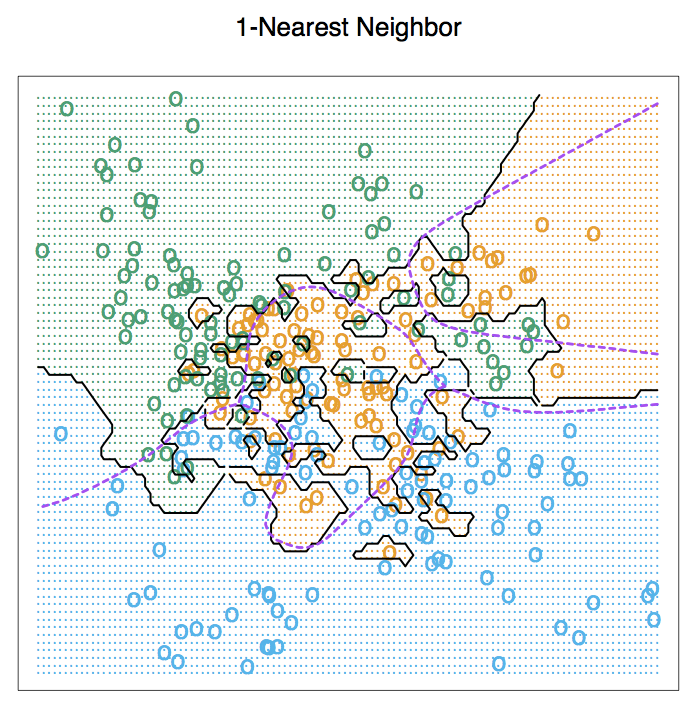
\includegraphics[height=0.8\textheight]{13_3_2.png}
\end{center}
\end{frame}

\begin{frame}{Сколько точек выбрать II}
\begin{center}
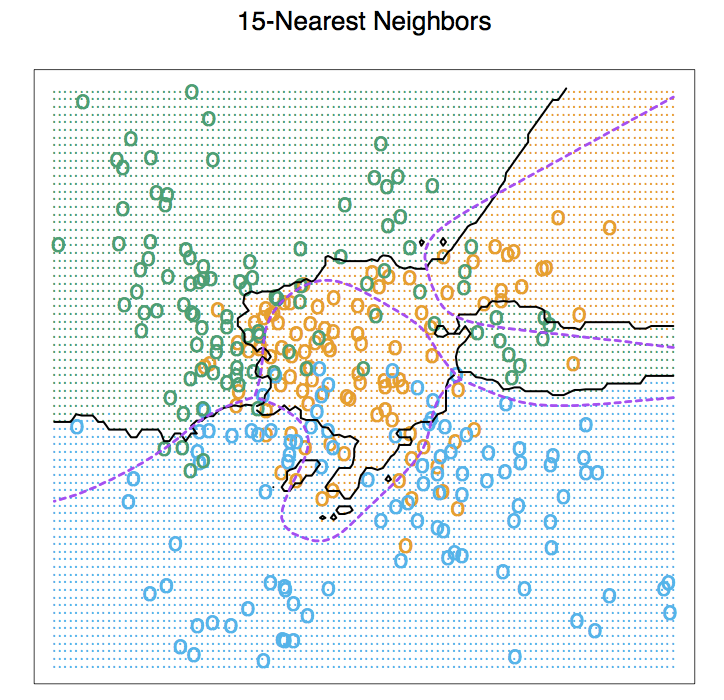
\includegraphics[height=0.8\textheight]{13_3_1.png}
\end{center}
\end{frame}


\begin{frame}{Свойства k-NN}
  \begin{itemize}
    \item Очень часто работает! 
    \item Простота реализации и наглядность.
    \item Ничего не требует на стадии обучения.
    \item Известная оценка сверху эффективности при отсутствии bias'а в learn'е. \\
    $$
      \begin{array}{l}
      BE = 1 - p(x|k^*) \\
      E = \sum_{i=1}^Kp(x|k)(1-p(x|k)) \\
      BE \le E \le 2BE \\
      \end{array}
    $$
    \item Часто требователен на фазе решения (!)
  \end{itemize}
\end{frame}


\begin{frame}{Основные способы прототипирования}
  Может много точек и не надо? Будет быстрее работать, глаже границы. \\
  Как выбрать прототипные точки:
  \begin{itemize}
    \item выбрать рандомно;
    \item покластеризовать каждый класс(например k-means'ами) и назначить центроиды прототипами;
    \item выбрать как-нибудь точки и подвигать их подальше от границ классов.
  \end{itemize}
\end{frame}

\begin{frame}{Learning Vector Quantization}
\begin{enumerate}
   \item построить вашим любимым методом прототипные точки;
   \item до сходимости уменьшая $\epsilon$ (learning rate): 
    \begin{enumerate}
      \item Случайно, равномерно выберем точку $x$ из learn'а с возвращением
      \item Найдём ближайший прототип
      \begin{description}
        \item [\color{blue}прототип нужного класса:] подвинем его ближе \\
        $ m_j^{t+1} = m_j^t + \epsilon (x - m_j^t)$ \\
        \item [\color{blue}"чужой" прототип:] подвинем его подальше \\
        $ m_j^{t+1} = m_j^t - \epsilon (x - m_j^t)$
      \end{description}
    \end{enumerate}
\end{enumerate}
\end{frame}

\begin{frame}{Проклятье размерности}
\emph{Что происходит с расстояниями когда размерность увеличивается?} \\
Проведем простой опыт: будем равномерно выбирать точки из кубика $[0, 1]^n \subset \mathbb{R}$. \\
Оказывается, что при увеличении $n$:
\begin{itemize}
  \item Точки все ближе “жмутся” к краю
  \item Углы между точками выравниваются
  \item Окрестности все чаще упираются в границы
  \item Для того, чтобы пространство было плотным надо слишком много точек
\end{itemize}
$\Rightarrow$ Большая размерность — зло для kNN и не только для него!
\end{frame}


\begin{frame}{Discriminant Adaptive Nearest-Neighbor (DANN)}
\small
\emph{Идея: а давайте в расстоянии учитывать локальную топологию в искомой точке}
Выберем много ближайших соседей (например m=50): \\
$$
  \begin{array}{l}
    T = m\Sigma = \sum_{i=1}^m(x_i - \mu(x))(x_i - \mu(x))^T \\
    = \sum_{k=1}^K \sum_{i \in I_k} (xi - \mu_k(x))(xi - \mu_k(x))^T \\
    + \sum_{k=1}^K(\mu_k(x) - \mu(x))(\mu_k(x) - \mu(x))^T \\ 
    = W + B
  \end{array}
$$
Пересчитаем все расстояния для k-NN:
$$
  \begin{array}{l}
    D(x, x_0) = (x - x_0)^T \mathcal{D}(x - x_0) \\
    \mathcal{D}=W^{-\frac{1}{2}} (W^{-\frac{1}{2}} B W^{-\frac{1}{2}} + \epsilon E) W^{-\frac{1}{2}}
  \end{array}
$$
Заметим, что ранги матриц, которые мы используем не более $m$. Получается очень точный, но крайне медленный метод.
\end{frame}

\begin{frame}{DANN результат}
\begin{center}
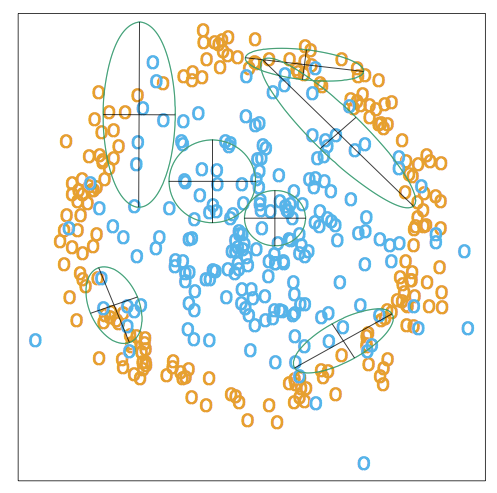
\includegraphics[height=0.8\textheight]{13_4.png}
\end{center}
\end{frame}

\begin{frame}{Поиск ближайших соседей}
  Это область на годовой курс, так что за поллекции мы ничего не успеем :).
  \begin{itemize}
    \item Линейный поиск
    \item Разбиение пространства
    \item Чувствительное к локальности хеширование (LSH)
    \item Кластерный/Пожатый поиск
    \item Деревья в пространстве меньшей размерности
  \end{itemize}
\end{frame}

\begin{frame}{kd-дерево}
  Идея: разложим множество по поторому будем искать в бинарное дерево с простыми условиями и конкретными точками в узлах. Будем надеяться на правило треугольника (не подходит для cosine(!)) \\
  Некоторые свойства:
  \begin{itemize}
    \item Один из самых простых способов поиска ближайших соседей
    \item Работает только в малых размерностях
    \item Затратные алгоритмы перестроения (если нужна динамика смотрим R-деревья)
  \end{itemize}  
\end{frame}

\begin{frame}{kd-дерево: построение}
\begin{enumerate}
  \item По циклу, или рандомно выбираем ось.
  \item Ищем точку, разбивающую множество на как можно более равные части.
  \item Повторяем 1-2 для каждого из получившихся подмножеств
\end{enumerate}
Сложность: $O(n \log n)$
\end{frame}

\begin{frame}{kd-дерево: построение (в картинках)}
\begin{center}
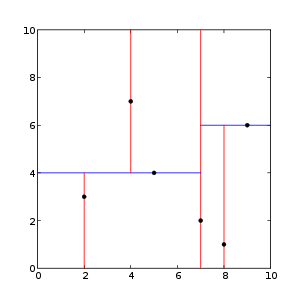
\includegraphics[height=0.9\textheight]{300px-Kdtree_2d.png}
\end{center}
\end{frame}

\begin{frame}{kd-дерево: поиск}
\begin{enumerate}
  \item Бежим по бинарному дереву поиска
  \item Когда добежали, сохраняем листовую точку как $\bar{x}$ - текущую лучшую
  \item Бежим обратно вверх по дереву:
  \begin{enumerate}
    \item если текущая точка лучше то теперь она $\bar{x}$;
    \item сравниваем расстояние от точки-запроса до гиперплоскости текущего уровня
    \begin{description}
      \item [\color{blue}пересекает:] не повезло, бежим в поддерево
      \item [\color{blue}не пересекает:] повезло, бежим наверх  
    \end{description}
  \end{enumerate}
  \item Повторяем 1-3 для каждого из получившихся подмножеств пока делятся
\end{enumerate}
Сложность сильно зависит от множества: в лучшем случае $O(\log n)$, в худшем $O(nN^{1-\frac{1}{n}})$ Классический пример проклятия размерности.
\end{frame}

\begin{frame}{kd-дерево: поиск (в картинках)}
\begin{center}
\animategraphics[width=0.9\textwidth,autoplay,loop]{0.3}{animate}{0}{5}
\end{center}
\end{frame}

\begin{frame}{kd-дерево: свойства}
\begin{enumerate}
  \item Необходимо правило треугольника
  \item Исходит из одинаковости направлений
  \item Работает только в малых размерностях.
\end{enumerate}
$\Rightarrow$ точно искать в реальных условиях не получается, будем неточно
\end{frame}

\begin{frame}{Немного определений}
\small
\begin{description}
  \item [\color{blue}Рандомизированнный $R$-ближайший сосед] если есть $R$-соседи, то алгоритм должен вернуть каждого из них с вероятностью $1 - \delta$
  \item [\color{blue}Р-я $c$-аппроксимация $R$-ближайшего соседа $((c , R ) - NN )$] если есть $R$-сосед, то алгоритм должен вернуть хотя бы одного $cR$-соседа с вероятностью $1 - \delta$
\end{description}
\end{frame}

\begin{frame}{Locality-Sensitive Hash Functions}
$\mathcal{H} = \{h|h: \mathbb{R}^n \to \mathbb{Z}_+\}, (R,cR,p_1,p_2):$
$$\begin{array}{l}
  \|p-q\| \le R \Rightarrow p_{\mathcal{H}}(h(p)=h(q)) \ge p_1 \\
  \|p-q\| \ge R \Rightarrow p_{\mathcal{H}}(h(p)=h(q)) \le p_2
\end{array}$$
Понятно, что хотим $p_1 > p_2$
\end{frame}


\begin{frame}{LSH алгоритм}
\small
Построение:
\begin{enumerate}
  \item Выберем $L$-функций семейства $\mathcal{H}^k$
  \item Поделим все данные на кусочки с одинаковыми значениями $g_i = (h_{i,1},...,h_{i,k})$
\end{enumerate}
Поиск по точке $q$:
\begin{enumerate}
  \item Выкинем $j \sim U\{1,...,L\}$
  \item Найдем значение $L_j(q)$ и соответствующий этому значению “кусочек”
  \item Линейно поищем в “кусочке”
  \item Одно из двух:
  \begin{enumerate}
    \item повторим 1-3 пока не найдется $L'$ точек (включая дубли) ближе чем $R$.
    \item переберём все $L$-функций.
  \end{enumerate}
\end{enumerate}
\end{frame}


\begin{frame}{Свойства LSH}
\begin{mydescription}{Первая стратегия}
  \item [\color{blue}Первая стратегия] с $L' = 3L$, для любой пары $(R, \delta), \exists L = O(N^{\frac{\ln p_1}{\ln p_2}} )$, гарантирующий $(c,R)-NN$
  \item [\color{blue}Вторая стратегия] гарантирует рандомизированного $R$ ближайшего соседа при $\delta = \delta(k, L)$
\end{mydescription}
\end{frame}

\begin{frame}{Некоторые известные семейства функций}
\begin{mydescription}{косинусная мера}
  \item [\color{blue}$l_1$] возьмём $w >> R, s_i \sim U[0, w], i=1,...,n$,
  $$
    h_{s_1,...,s_n} = (\left[\frac{(x_1 - s_1)}{w}\right], ..., \left[\frac{(x_n - s_n)}{w}\right])
  $$
  \item [\color{blue}$l_s$] возьмём $w >> R, r_i \sim N(0, 1), h_{w, r, b} = [\frac{r^Tx+b}{w}]$ при $\delta = \delta(k, L)$
  \item [\color{blue}косинусная мера] возьмём $r_i\sim N(0,1), h_r = sign(x,r)$
\end{mydescription}
\end{frame}

\begin{frame}{Что мы сегодня узнали}
\begin{itemize}
  \item Instance based learning
    \begin{itemize}
      \item Иногда можно использовать learn в качестве решающей функции
      \item Есть проклятье размерности, которое нам мешает
      \item Можно учитывать проклятье при построении метода
    \end{itemize}
  \item Поиск ближайших соседей
  \begin{itemize}
    \item Это большая область
    \item Если размерность мелкая и есть правило треугольника, то можно искать точно (kd-tree, r-tree)
    \item Можно искать неточно, но с гарантиями (LSH)
  \end{itemize}
\end{itemize}
\end{frame}

\end{document}
